\section{Extended partitioning: format partitions}
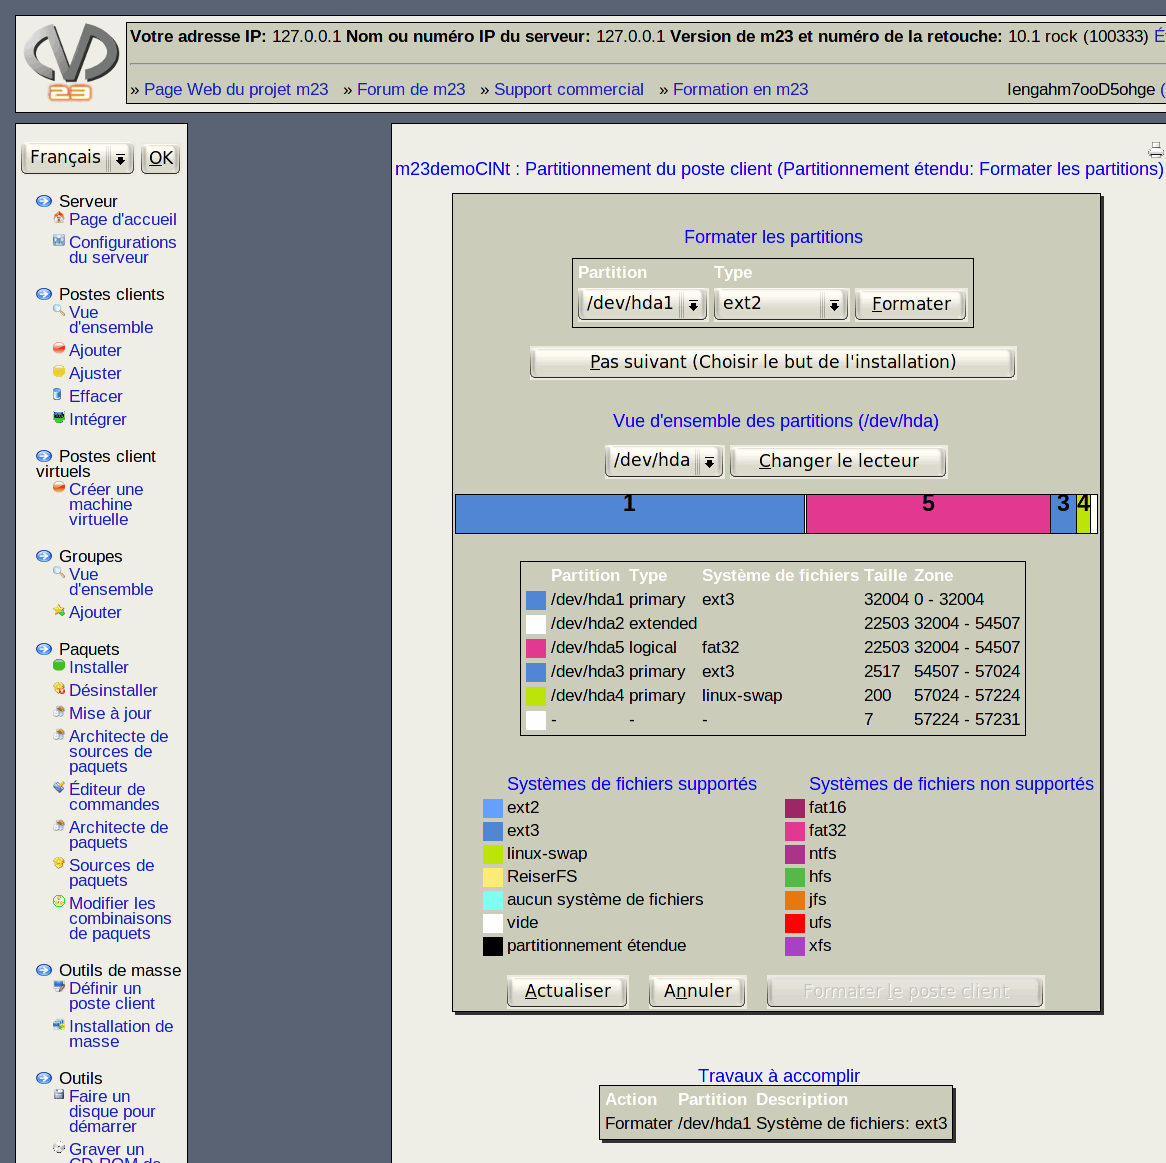
\includegraphics[scale=0.4]{/mdk/doc/manual/screenshots/en/fdisk-extended2.png} \\
\begin{enumerate}
\item Select the partition you want to format, choose the file system type and click on \textit{"Format"}. You can see additional information about possible file systems at the bottom of the page.\\
\item Click on \textit{""} when you have formatted all desired partitions.\\
\end{enumerate}
\subsection{Hint}
You need at least one ext2, ext3 or reiserfs formatted and one linux-swap formatted partition to begin the installation.\\
\subsection{Information: File systems}
\begin{itemize}
\item \textbf{ext2}: An old but seldom used file system that can be used to install the base system on it.\\
\item \textbf{ext3(recommended), reiserfs}: newer journalling file systems, that can be used to install the base system on.\\
\item \textbf{linux-swap}: is used as the swap space.\\
\end{itemize}
